\section{Known Bugs}
Im Rahmen der Entwicklung und mit Fortschreiten des Projekts sind, trotz Reviews der einzelnen Elemente des Projekts, Fehler bekannt geworden, die komplett oder teilweise gelöst oder umgangen wurden. Auf diese Fehler wird in den folgenden Abschnitten eingegangen.
\subsection{Hardware}
Bei der Hardwareentwicklung sind schaltungstechnisch und bzgl. der erstellten Bauteilbibliothek Fehler aufgetreten. 
\subsubsection{HDMI-Stecker gekreuzt}
\textbf{Problem:} Im Schaltplanprogramm \code{Eagle} wurde durch einen Fehler beim Erstellen der HDMI-Buchse CON2 fälschlicherweise die Belegung des Steckers verwendet. Die Verwendung von normalen HDMI-Kabeln ist daher nicht möglich!\\
\textbf{Workaround:} Alle Signale müssen gekreuzt werden. Hierzu wird ein HDMI-Stecker an ein abgetrenntes Ende eines HDMI-Kabels angelötet. Die Belegung wird entsprechend \refa{fig:hdmi_stecker_problem}\footnote{Quelle: \url{http://de.wikipedia.org/wiki/Datei:HDMI_Connector_Pinout.svg}} gekreuzt.
\begin{figure}[htp]
	\center
	\fbox{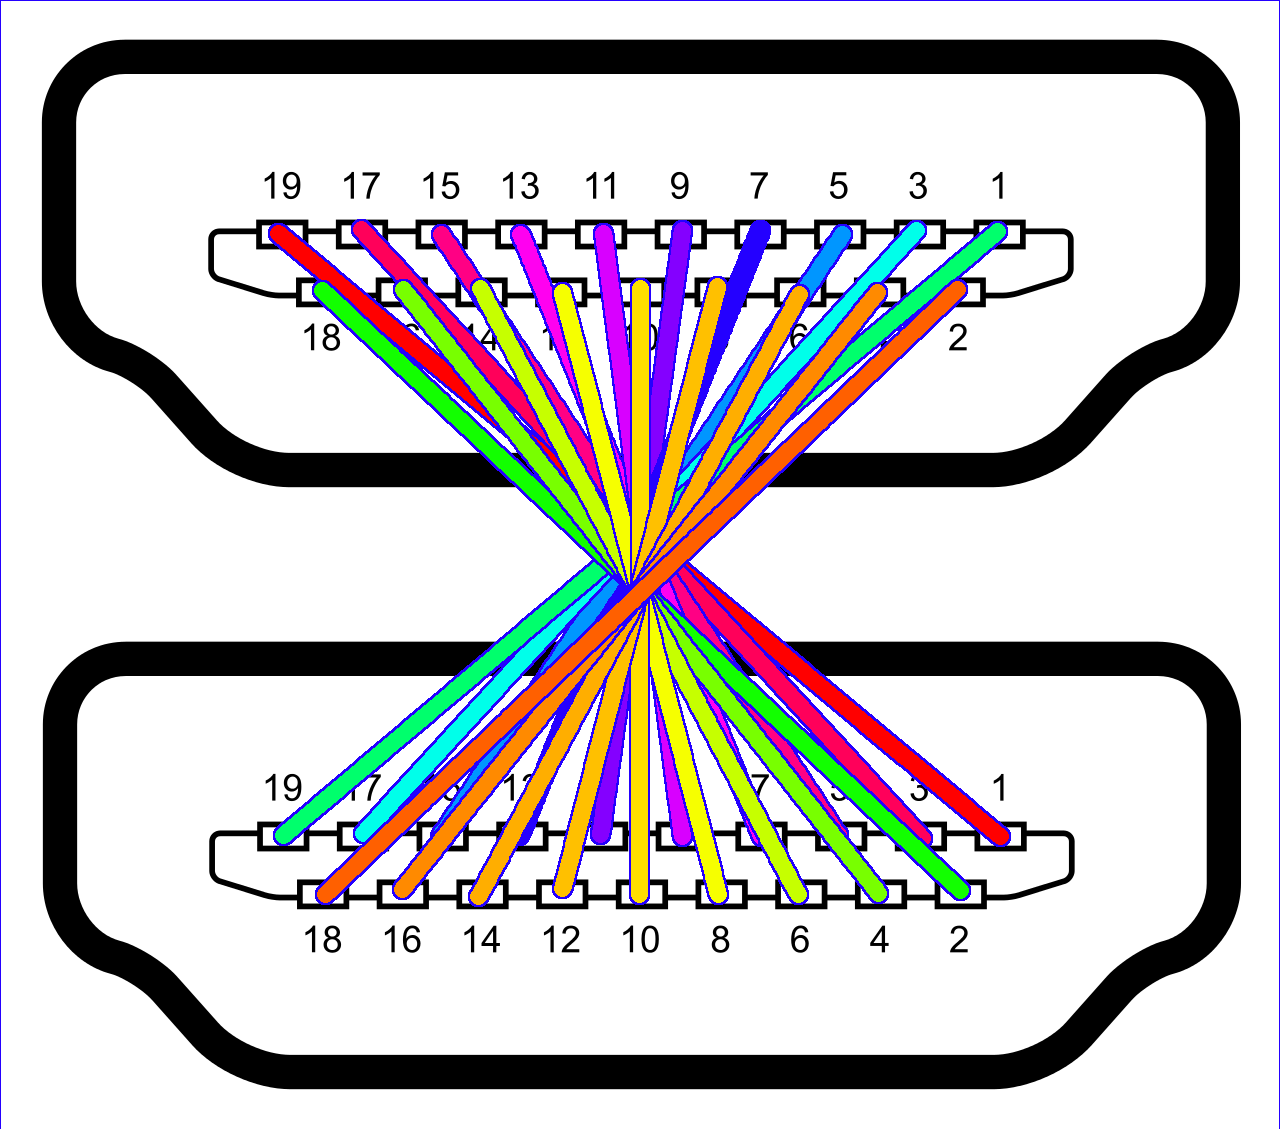
\includegraphics[width=0.6\textwidth]{TeilB/hdmi_stecker_problem.png}}
    \caption{Known Bugs: HDMI-Stecker}
    \label{fig:hdmi_stecker_problem}
\end{figure}\\
%    }}
\textbf{Lösung:} Um das Problem endgültig zu lösen, muss das Schaltplansymbol in \code{Eagle}\\sowie das Platinenlayout bei der Beschaltung der HDMI-Buchse und der RGB-Bridge angepasst werden.
\subsubsection{LVDS-Steckerfootprint gespiegelt}
\textbf{Problem:} Das Schaltplansymbol des LVDS-Steckers CON6 muss gespiegelt werden. Das Anstecken des LVDS-Displays mit vorgesehener Belegung kann zu Beschädigung des Displays führen.\\
\textbf{Workaround:} Der LVDS-Stecker wird um 180 Grad gedreht auf die bereits dort vorgesehenen Pads angelötet.\\
\textbf{Lösung:} Das Schaltplansymbol muss in \code{Eagle} um 180 Grad gedreht werden.
\subsubsection{+5V-Kreis}
\textbf{Problem:} Der Widerstand \code{R13} wird verwendet um eventuell auftretende Spannungsunterschiede zwischen den +5\,V der USB- und HDMI-Versorgung auszugleichen (siehe \refa{fig:r13}). Dieser Widerstand ist mit 10\,k$\Omega$ zu groß gewählt.
\begin{figure}[htp]
	\center
	\fbox{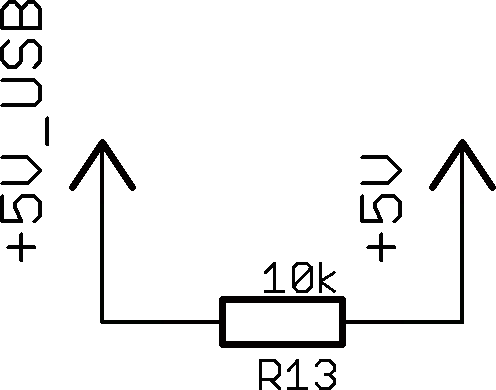
\includegraphics[width=0.2\textwidth]{TeilB/r13.png}}
    \caption{Known Bugs: +5V-Kreis}
    \label{fig:r13}
\end{figure}\\
\textbf{Lösung:} Verkleinerung des Widerstands bzw. Entfernen und Überbrücken von \code{R13} mit 0\,$\Omega$.
\subsubsection{USB D+/D- vertauscht}
\textbf{Problem:} Die USB-Datensignale \code{USB_D+} und \code{USB_D-} sind vertauscht (siehe \refa{fig:usb_vertauscht}). Dies verhindert die Kommunikation zwischen PC und AVR.
\begin{figure}[htp]
	\center
	\fbox{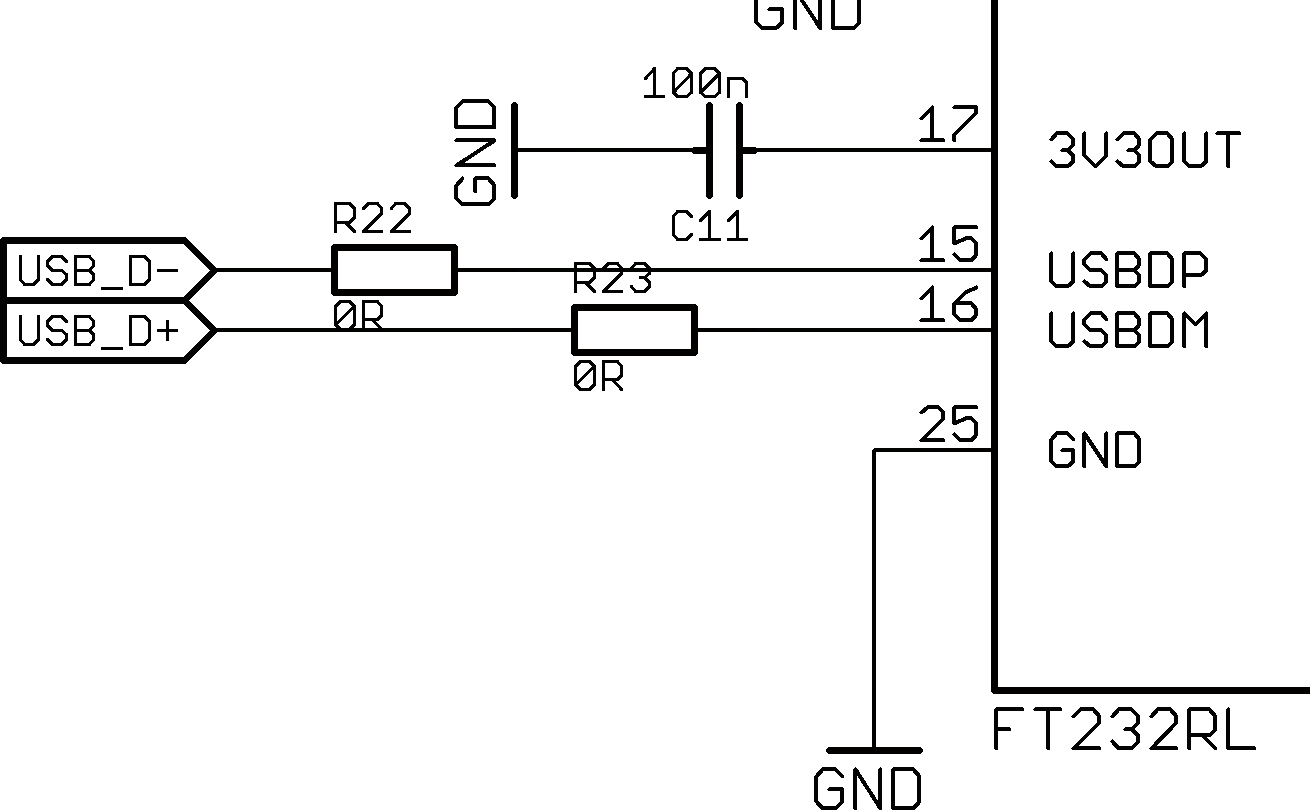
\includegraphics[width=0.45\textwidth]{TeilB/usb_dp_dm.png}}
    \caption{Known Bugs: USB Signale vertauscht}
    \label{fig:usb_vertauscht}
\end{figure}\\
\textbf{Workaround:} Entfernen der 0\,$\Omega$ Widerstände \code{R22} und \code{R23} und kreuzen der Signale mit Fädeldraht.\\
\textbf{Lösung:} Um das Problem endgültig zu beheben, müssen die Signale \code{USB_D+} und \code{USB_D-} im Schaltplan am Baustein \code{FT232RL} getauscht und im Platinenlayout entsprechende Anpassungen gemacht werden.
\subsection{Software}
\textbf{Problem:} Unter bisher ungeklärten Umständen kann es vorkommen, dass die Prüfsumme des ausgelesenen EEPROMs und der im PC-Programm berechneten Software nicht übereinstimmt. \\
\textbf{Workaround:} Ein erneuter Programmiervorgang umgeht das Problem. Die Prüfsummen werden korrekt berechnet und verglichen.